\documentclass[9pt,twocolumn,twoside]{../../styles/osajnl}
\usepackage{fancyvrb}
\journal{i524} 

\title{Introduction to Terraform}

\author[1]{Sushmita Sivaprasad}


\affil[1]{School of Informatics and Computing, Bloomington, IN 47408, U.S.A.}


\affil[*]{Corresponding authors: sushsiva@umail.iu.edu}

\dates{project-000, \today}

\ociscodes{Terraform, IAC, Go code, Ansible}

% replace this with your url in github/gitlab
\doi{\url{https://github.com/cloudmesh/sp17-i524/tree/master/paper2/S17-IR-2038/report.pdf}}


\begin{abstract}
This paper gives a brief introduction on Terraform and how
infrastructure can be used as a code , which is the building block
of Terrform. It is written in go scripting code and it is a server
provisioning tool where we can specify what is the goal we require
and Terraform creates steps of tasks on how to reach the goal. This
paper provides information on what are the use cases of Terrform and
how it differentiates itself from other tools. Resources for
learning Terraform in much more detail has been referenced as well.
  
\end{abstract}

\setboolean{displaycopyright}{true}

\begin{document}

\maketitle

\section{1.Introduction}

Terraform is an open source tool created by HashiCorp. It is an
infrastructure management tool written in Go programming language.It
allows users to safely and predictably create , change and improve the
production infrastructure and codifies the API's into a declarative
configuration file that can be shared among other users as
well\cite{www-terraform}. The tool can even be treated as a code
whereby we can edit , review and create versions at the same time. The
tool is popular is allowing users to create customized in-house
solutions. It allows to build an executive plan which can be used for
the purpose of creating applications and for the purpose of
implementing the infrastructure\cite{www-terraform-book}.

\section{2.Infrastructure as a code}

Infrastructure as a code or IAC allows us to write and execute a code
in order to define, deploy and update the infrastructure. There are 4
categories of the IAC tools ,
\subsection{2.1.Ad hoc scripts}

Ad Hoc scripts allows to automate anything. We can use any scripting
language and break down the tasks we were doing manually and execute
the script on the server. Ad hoc script allows one to write the code
is however manner required\cite{www-terraform-upandrunning}

\subsection{2.2.Configuration management tools}

Some of the main configuration management tools are Chef, Ansible ,
SaltStack which are desgined to install and manage software on any of
the existing servers. These tools are designed to managed a large
number of remote servers.Ansible playbook can be used to configure
multiple servers in a parallel mode. A parameter called as serial can
be set in the playbook from which a rolling deployement can be done
and the server will be updated batch wise. Tools such as Ansible are
idempotent, that is they run correctly no matter how many times we run
the code\cite{www-terraform-upandrunning}

\subsection{2.3.Server templating tools}
Server templating tools are Docker, Packer and Vagrant. A server
templating tool allows to create an image of a server that captures a
snapshot image of the operating system, the software and the files in
it. The image of the server can then be distributed across all of the
servers using Ansible\cite{www-terraform-upandrunning}.


\begin{figure}[h]
  \begin{center}
 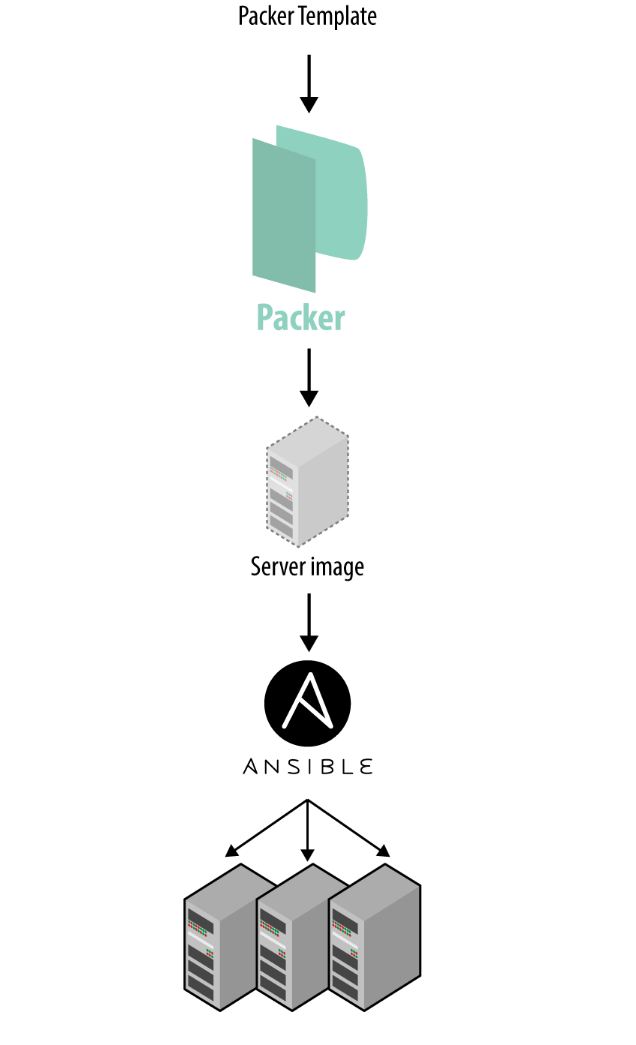
\includegraphics[width=\linewidth,height=4in]{images/packer}
 \caption{ Packer is used to create an image of a server which can be installed using Ansible across all other servers \cite{www-terraform-upandrunning}}
 \label{fig}
  \end{center}
\end{figure}

\subsection{2.4.Server provisioning tools}
Server provisioning tools includes Terraform , Cloudformation ,
Openstack Heat. These tools allows to create a server by
themselves. These tools can also be used to create databases, caches ,
load balancers, queues, firewall settings and other aspects from the
infrastructure\cite{www-terraform-upandrunning}.

\section{3.Working of Terraform}
Infrastructure is the building block on which the application is
created on.  Terraform provides us a declarative execution plan for
building and running applications and infrastructure. All that we are
required to do in a declarative state is we declare the required end
state. The tool will take care of the steps required to reach the goal
state. It allows the user to not be bothered about the commands to run
or the settings required to change.  The user has to declare the
resources using a graph-based approach in order to model and apply the
desired state\cite{www-terraform-book}.\\ The Go code allows Terraform
to compile down into a single binary code for each of the supported
operating systems.This binary is used to deploy infrastructure from
our pc or a server and we would not require an additional
infrastructure to make that happen.The binary makes API calls on
behalf of us to one or more of the providers such as Azure , AWS ,
Google Cloud,etc. In this way terraform lets users to use the
infrastructures provided by these providers as well as the
authentication mechanism we are already using with these providers
\cite{www-terraform-upandrunning}. Terraform allows users to deploy
interconnected resources across various cloud providers at the same
time. It translates the contents of the configurations into API calls
into the cloud providers as shown in figure 2.


\begin{figure}[h]
  \begin{center}
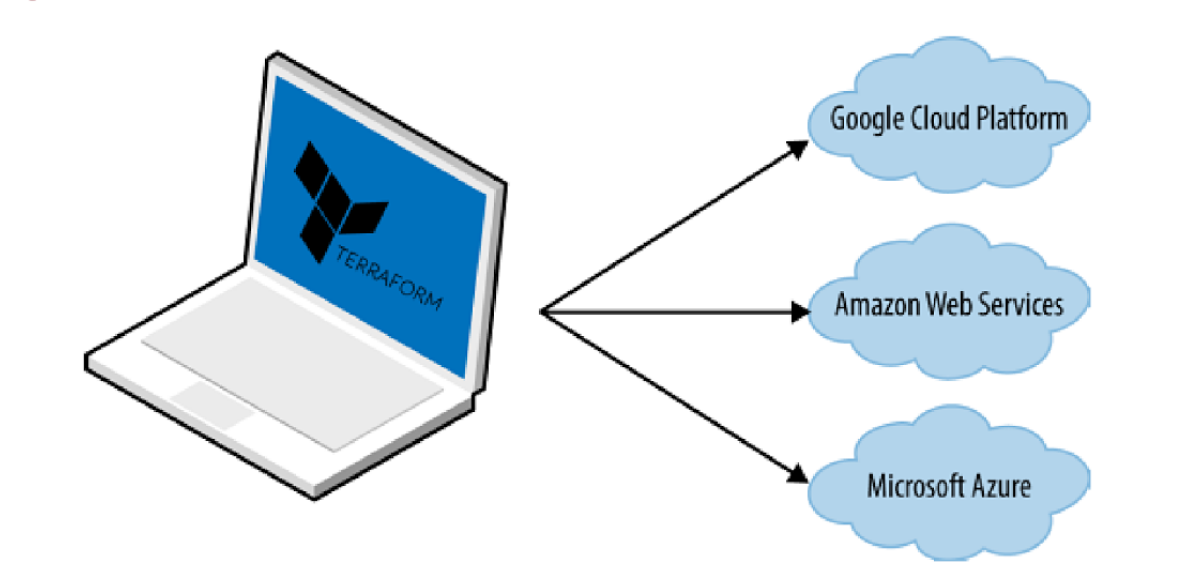
\includegraphics[width=\linewidth,height=3in]{images/terraform_1}
\caption{Figure depicting terraform transforming the configurations to
  API calls into the cloud providers \cite{www-terraform-book}}
\label{fig:work}
\end{center}
\end{figure}

\section{4.Use Cases}

\subsection{4.1.Multi-tier application}

It is useful for building multi-tier applicatin which consists of web,
cache, application, middleware and tiers of database.Terraform helps
to build N-tier applications. Each of the tier can be configured in
Terraform and left independent and isolated and can be easily scaled
and managed by the code\cite{www-terraform-book}.


\subsection{4.2.Disposable Environments}

In order to test a new application before it has been sent for
production , a staging or QA Environment is required in order to avoid
complexity and confusion. For such a situation terraform can be very
handy, where the production environment can be codified and shared
along with staging. It can even create new environment for it to test
on and which can be later disposed of , keeping only what is
required. Terraform makes it easy to maintain paralle environements
and easily dispose them of\cite{www-terraform-book}.

\subsection{4.3. Multi-Cloud Deployment}

In order to increase the fault tolerance , infrastructure is spread
across multiple clouds to continue it's progress irrespective of any
faults. The current multi-cloud deployement consists of cloud specific
tools for infrastructure management. Terraform allows a single
configuration to be used across multiple providers and also handle any
cross-cloud dependencies\cite{www-terraform}.

\section{5.Advantages of using Terraform}

Terraform allows the existing tools to focus on its strength such as
bootstrapping and initializing resources. It makes the infrastructure
deployment easy by focusing on a higher level of abstraction of the
datacenter and also allowing the same codification for the tools. It
is cloud agnostic and allows multiple providers and services to be
combined. It separates the planning and execution phase. It generates
an action plan when we provide a goal state, which keeps getting
updated when we add or remove new resources. The terraform graph
feature allows the user to visualize the plan in order for them to
know exactly the effects of the changes before they get implemented
\cite{www-terraform-othersoftware}.

\section{6.Educational material}

Hashicorp has provided a documentation for describing Terraform , it's
download and installation procedure. There has been 2 books published
by authors Yevgeniy Brikman\cite{www-terraform-upandrunning} James
Turnbull\cite{www-terraform-book} which gives a very detailed insight
about the working and usage of Terraform.

\section{7.Conclusion}
Terraform simplifies the process of creating applications and
implementing the infrastructure by just specifying the required
goal. It uses Go code which allows Terraform to compile down into a
single binary code for each of the supported operating systems. We can
create N- tier applications with ease by just providing the resources
and the end state of the required application. It allows multiple user
to work on a cloud-agnostic platform thus being a very versatile tool.

\section*{Acknowledgements}
The author is grateful to the School of Informatics and Computing for
providing an opportunity to work on the paper. The author is thankful
to Prof Gregor Laszewski and the teaching assistants for all the
prompt technical support.

\bibliography{references}

\section{Author Biography}

{\bfseries Sushmita Sivaprasad} received her B.E in ELectronics and
Communication from SRM University, Chennai, India and her M.S in
International Business from Hult International Business School, Dubai,
UAE. She is currently pursuing her graduate studies in Data Science in
Indiana University Bloomington.

\end{document}
